% Options for packages loaded elsewhere
\PassOptionsToPackage{unicode}{hyperref}
\PassOptionsToPackage{hyphens}{url}
%
\documentclass[
  spanish,
]{article}
\usepackage{lmodern}
\usepackage{setspace}
\usepackage{amssymb,amsmath}
\usepackage{ifxetex,ifluatex}
\ifnum 0\ifxetex 1\fi\ifluatex 1\fi=0 % if pdftex
  \usepackage[T1]{fontenc}
  \usepackage[utf8]{inputenc}
  \usepackage{textcomp} % provide euro and other symbols
\else % if luatex or xetex
  \usepackage{unicode-math}
  \defaultfontfeatures{Scale=MatchLowercase}
  \defaultfontfeatures[\rmfamily]{Ligatures=TeX,Scale=1}
  \setmainfont[]{Open Sans}
  \setmonofont[]{Fira Code Light}
\fi
% Use upquote if available, for straight quotes in verbatim environments
\IfFileExists{upquote.sty}{\usepackage{upquote}}{}
\IfFileExists{microtype.sty}{% use microtype if available
  \usepackage[]{microtype}
  \UseMicrotypeSet[protrusion]{basicmath} % disable protrusion for tt fonts
}{}
\makeatletter
\@ifundefined{KOMAClassName}{% if non-KOMA class
  \IfFileExists{parskip.sty}{%
    \usepackage{parskip}
  }{% else
    \setlength{\parindent}{0pt}
    \setlength{\parskip}{6pt plus 2pt minus 1pt}}
}{% if KOMA class
  \KOMAoptions{parskip=half}}
\makeatother
\usepackage{xcolor}
\IfFileExists{xurl.sty}{\usepackage{xurl}}{} % add URL line breaks if available
\IfFileExists{bookmark.sty}{\usepackage{bookmark}}{\usepackage{hyperref}}
\hypersetup{
  pdftitle={Manual KTensorGraph},
  pdfauthor={José Miguel Hernández Cabrera},
  pdflang={es},
  hidelinks,
  pdfcreator={LaTeX via pandoc}}
\urlstyle{same} % disable monospaced font for URLs
\usepackage[margin=1in]{geometry}
\usepackage{color}
\usepackage{fancyvrb}
\newcommand{\VerbBar}{|}
\newcommand{\VERB}{\Verb[commandchars=\\\{\}]}
\DefineVerbatimEnvironment{Highlighting}{Verbatim}{commandchars=\\\{\}}
% Add ',fontsize=\small' for more characters per line
\usepackage{framed}
\definecolor{shadecolor}{RGB}{248,248,248}
\newenvironment{Shaded}{\begin{snugshade}}{\end{snugshade}}
\newcommand{\AlertTok}[1]{\textcolor[rgb]{0.94,0.16,0.16}{#1}}
\newcommand{\AnnotationTok}[1]{\textcolor[rgb]{0.56,0.35,0.01}{\textbf{\textit{#1}}}}
\newcommand{\AttributeTok}[1]{\textcolor[rgb]{0.77,0.63,0.00}{#1}}
\newcommand{\BaseNTok}[1]{\textcolor[rgb]{0.00,0.00,0.81}{#1}}
\newcommand{\BuiltInTok}[1]{#1}
\newcommand{\CharTok}[1]{\textcolor[rgb]{0.31,0.60,0.02}{#1}}
\newcommand{\CommentTok}[1]{\textcolor[rgb]{0.56,0.35,0.01}{\textit{#1}}}
\newcommand{\CommentVarTok}[1]{\textcolor[rgb]{0.56,0.35,0.01}{\textbf{\textit{#1}}}}
\newcommand{\ConstantTok}[1]{\textcolor[rgb]{0.00,0.00,0.00}{#1}}
\newcommand{\ControlFlowTok}[1]{\textcolor[rgb]{0.13,0.29,0.53}{\textbf{#1}}}
\newcommand{\DataTypeTok}[1]{\textcolor[rgb]{0.13,0.29,0.53}{#1}}
\newcommand{\DecValTok}[1]{\textcolor[rgb]{0.00,0.00,0.81}{#1}}
\newcommand{\DocumentationTok}[1]{\textcolor[rgb]{0.56,0.35,0.01}{\textbf{\textit{#1}}}}
\newcommand{\ErrorTok}[1]{\textcolor[rgb]{0.64,0.00,0.00}{\textbf{#1}}}
\newcommand{\ExtensionTok}[1]{#1}
\newcommand{\FloatTok}[1]{\textcolor[rgb]{0.00,0.00,0.81}{#1}}
\newcommand{\FunctionTok}[1]{\textcolor[rgb]{0.00,0.00,0.00}{#1}}
\newcommand{\ImportTok}[1]{#1}
\newcommand{\InformationTok}[1]{\textcolor[rgb]{0.56,0.35,0.01}{\textbf{\textit{#1}}}}
\newcommand{\KeywordTok}[1]{\textcolor[rgb]{0.13,0.29,0.53}{\textbf{#1}}}
\newcommand{\NormalTok}[1]{#1}
\newcommand{\OperatorTok}[1]{\textcolor[rgb]{0.81,0.36,0.00}{\textbf{#1}}}
\newcommand{\OtherTok}[1]{\textcolor[rgb]{0.56,0.35,0.01}{#1}}
\newcommand{\PreprocessorTok}[1]{\textcolor[rgb]{0.56,0.35,0.01}{\textit{#1}}}
\newcommand{\RegionMarkerTok}[1]{#1}
\newcommand{\SpecialCharTok}[1]{\textcolor[rgb]{0.00,0.00,0.00}{#1}}
\newcommand{\SpecialStringTok}[1]{\textcolor[rgb]{0.31,0.60,0.02}{#1}}
\newcommand{\StringTok}[1]{\textcolor[rgb]{0.31,0.60,0.02}{#1}}
\newcommand{\VariableTok}[1]{\textcolor[rgb]{0.00,0.00,0.00}{#1}}
\newcommand{\VerbatimStringTok}[1]{\textcolor[rgb]{0.31,0.60,0.02}{#1}}
\newcommand{\WarningTok}[1]{\textcolor[rgb]{0.56,0.35,0.01}{\textbf{\textit{#1}}}}
\usepackage{longtable,booktabs}
% Correct order of tables after \paragraph or \subparagraph
\usepackage{etoolbox}
\makeatletter
\patchcmd\longtable{\par}{\if@noskipsec\mbox{}\fi\par}{}{}
\makeatother
% Allow footnotes in longtable head/foot
\IfFileExists{footnotehyper.sty}{\usepackage{footnotehyper}}{\usepackage{footnote}}
\makesavenoteenv{longtable}
\usepackage{graphicx}
\makeatletter
\def\maxwidth{\ifdim\Gin@nat@width>\linewidth\linewidth\else\Gin@nat@width\fi}
\def\maxheight{\ifdim\Gin@nat@height>\textheight\textheight\else\Gin@nat@height\fi}
\makeatother
% Scale images if necessary, so that they will not overflow the page
% margins by default, and it is still possible to overwrite the defaults
% using explicit options in \includegraphics[width, height, ...]{}
\setkeys{Gin}{width=\maxwidth,height=\maxheight,keepaspectratio}
% Set default figure placement to htbp
\makeatletter
\def\fps@figure{htbp}
\makeatother
\setlength{\emergencystretch}{3em} % prevent overfull lines
\providecommand{\tightlist}{%
  \setlength{\itemsep}{0pt}\setlength{\parskip}{0pt}}
\setcounter{secnumdepth}{-\maxdimen} % remove section numbering
\ifxetex
  % Load polyglossia as late as possible: uses bidi with RTL langages (e.g. Hebrew, Arabic)
  \usepackage{polyglossia}
  \setmainlanguage[]{spanish}
\else
  \usepackage[shorthands=off,main=spanish]{babel}
\fi
\newlength{\cslhangindent}
\setlength{\cslhangindent}{1.5em}
\newenvironment{cslreferences}%
  {\setlength{\parindent}{0pt}%
  \everypar{\setlength{\hangindent}{\cslhangindent}}\ignorespaces}%
  {\par}

\title{Manual KTensorGraph}
\usepackage{etoolbox}
\makeatletter
\providecommand{\subtitle}[1]{% add subtitle to \maketitle
  \apptocmd{\@title}{\par {\large #1 \par}}{}{}
}
\makeatother
\subtitle{Modelos para describir tablas de 3 entradas}
\author{José Miguel Hernández Cabrera}
\date{}

\begin{document}
\maketitle

\setstretch{1.15}
\hypertarget{introducciuxf3n}{%
\subsection{Introducción}\label{introducciuxf3n}}

Este es un manual sobre cómo realizar un flujo de trabajo con el paquete \texttt{KTensorGraph} desarrollado por Rodriguez-Rosa (2019) para utilizar la técnicas Tucker. En manual se centrarán en el Tucker-3, dado que con esta técnica se pueden detectar interacciones para la que se hayan retenido diferentes números de componentes para tres dimensiones. Asimismo, el flujo es reproducible ante cualquier otra técnica. Se recomienda revisar el trabajo de Rodrı́guez-Rosa et~al. (2018) para encontrar cálculos similares como referencia.

Los datos utilizados provienen de la investigación de Thioulouse et~al. (2004), en el cual los investigadores utilizaron el método STATICO para analizar una serie de tablas ecológicas pareadas de un áera geográfica de Francia, cuyos nombres se describen en la tabla \#. El par se compone de abundancia de especies del lugar\footnote{Cabe aclarar que algunas especies pueden estar ausentes en algunas tablas.} y variables ambientales. Las filas corresponden a los sitios muestrados, los cuales son los mismos en ambas tablas. Además, las tablas se repiten por cada estación del año.

\begin{longtable}[]{@{}llll@{}}
\caption{Descripción de especies y variables.}\tabularnewline
\toprule
\begin{minipage}[b]{0.12\columnwidth}\raggedright
Especies\strut
\end{minipage} & \begin{minipage}[b]{0.27\columnwidth}\raggedright
Descripción\strut
\end{minipage} & \begin{minipage}[b]{0.14\columnwidth}\raggedright
Variables\strut
\end{minipage} & \begin{minipage}[b]{0.35\columnwidth}\raggedright
Descripción\strut
\end{minipage}\tabularnewline
\midrule
\endfirsthead
\toprule
\begin{minipage}[b]{0.12\columnwidth}\raggedright
Especies\strut
\end{minipage} & \begin{minipage}[b]{0.27\columnwidth}\raggedright
Descripción\strut
\end{minipage} & \begin{minipage}[b]{0.14\columnwidth}\raggedright
Variables\strut
\end{minipage} & \begin{minipage}[b]{0.35\columnwidth}\raggedright
Descripción\strut
\end{minipage}\tabularnewline
\midrule
\endhead
\begin{minipage}[t]{0.12\columnwidth}\raggedright
Eda\strut
\end{minipage} & \begin{minipage}[t]{0.27\columnwidth}\raggedright
Ephemera danica\strut
\end{minipage} & \begin{minipage}[t]{0.14\columnwidth}\raggedright
Temp.\strut
\end{minipage} & \begin{minipage}[t]{0.35\columnwidth}\raggedright
Temperatura\strut
\end{minipage}\tabularnewline
\begin{minipage}[t]{0.12\columnwidth}\raggedright
Bsp\strut
\end{minipage} & \begin{minipage}[t]{0.27\columnwidth}\raggedright
Baetis sp.\strut
\end{minipage} & \begin{minipage}[t]{0.14\columnwidth}\raggedright
Flow\strut
\end{minipage} & \begin{minipage}[t]{0.35\columnwidth}\raggedright
Flujo\strut
\end{minipage}\tabularnewline
\begin{minipage}[t]{0.12\columnwidth}\raggedright
Brh\strut
\end{minipage} & \begin{minipage}[t]{0.27\columnwidth}\raggedright
Baetis rhodani\strut
\end{minipage} & \begin{minipage}[t]{0.14\columnwidth}\raggedright
pH\strut
\end{minipage} & \begin{minipage}[t]{0.35\columnwidth}\raggedright
\strut
\end{minipage}\tabularnewline
\begin{minipage}[t]{0.12\columnwidth}\raggedright
Bni\strut
\end{minipage} & \begin{minipage}[t]{0.27\columnwidth}\raggedright
Baetis niger\strut
\end{minipage} & \begin{minipage}[t]{0.14\columnwidth}\raggedright
Conduct.\strut
\end{minipage} & \begin{minipage}[t]{0.35\columnwidth}\raggedright
Conductividad\strut
\end{minipage}\tabularnewline
\begin{minipage}[t]{0.12\columnwidth}\raggedright
Bpu\strut
\end{minipage} & \begin{minipage}[t]{0.27\columnwidth}\raggedright
Baetis pumilus\strut
\end{minipage} & \begin{minipage}[t]{0.14\columnwidth}\raggedright
Oxygen\strut
\end{minipage} & \begin{minipage}[t]{0.35\columnwidth}\raggedright
Oxígeno\strut
\end{minipage}\tabularnewline
\begin{minipage}[t]{0.12\columnwidth}\raggedright
Cen\strut
\end{minipage} & \begin{minipage}[t]{0.27\columnwidth}\raggedright
Centroptilum\strut
\end{minipage} & \begin{minipage}[t]{0.14\columnwidth}\raggedright
BDO5\strut
\end{minipage} & \begin{minipage}[t]{0.35\columnwidth}\raggedright
Demanda biológica por oxígeno\strut
\end{minipage}\tabularnewline
\begin{minipage}[t]{0.12\columnwidth}\raggedright
Ecd\strut
\end{minipage} & \begin{minipage}[t]{0.27\columnwidth}\raggedright
Ecdyonurus\strut
\end{minipage} & \begin{minipage}[t]{0.14\columnwidth}\raggedright
Oxydab.\strut
\end{minipage} & \begin{minipage}[t]{0.35\columnwidth}\raggedright
Oxidabilidad\strut
\end{minipage}\tabularnewline
\begin{minipage}[t]{0.12\columnwidth}\raggedright
Rhi\strut
\end{minipage} & \begin{minipage}[t]{0.27\columnwidth}\raggedright
Rhithrogena\strut
\end{minipage} & \begin{minipage}[t]{0.14\columnwidth}\raggedright
Ammo.\strut
\end{minipage} & \begin{minipage}[t]{0.35\columnwidth}\raggedright
Amonio\strut
\end{minipage}\tabularnewline
\begin{minipage}[t]{0.12\columnwidth}\raggedright
Hla\strut
\end{minipage} & \begin{minipage}[t]{0.27\columnwidth}\raggedright
Habrophlebia lauta\strut
\end{minipage} & \begin{minipage}[t]{0.14\columnwidth}\raggedright
Nitrates\strut
\end{minipage} & \begin{minipage}[t]{0.35\columnwidth}\raggedright
Nitratos\strut
\end{minipage}\tabularnewline
\begin{minipage}[t]{0.12\columnwidth}\raggedright
Hab\strut
\end{minipage} & \begin{minipage}[t]{0.27\columnwidth}\raggedright
Habroletoides modesta\strut
\end{minipage} & \begin{minipage}[t]{0.14\columnwidth}\raggedright
Phosps.\strut
\end{minipage} & \begin{minipage}[t]{0.35\columnwidth}\raggedright
Fosfato\strut
\end{minipage}\tabularnewline
\begin{minipage}[t]{0.12\columnwidth}\raggedright
Par\strut
\end{minipage} & \begin{minipage}[t]{0.27\columnwidth}\raggedright
Paraletophlebia\strut
\end{minipage} & \begin{minipage}[t]{0.14\columnwidth}\raggedright
\strut
\end{minipage} & \begin{minipage}[t]{0.35\columnwidth}\raggedright
\strut
\end{minipage}\tabularnewline
\begin{minipage}[t]{0.12\columnwidth}\raggedright
Cae\strut
\end{minipage} & \begin{minipage}[t]{0.27\columnwidth}\raggedright
Caenis\strut
\end{minipage} & \begin{minipage}[t]{0.14\columnwidth}\raggedright
\strut
\end{minipage} & \begin{minipage}[t]{0.35\columnwidth}\raggedright
\strut
\end{minipage}\tabularnewline
\begin{minipage}[t]{0.12\columnwidth}\raggedright
Eig\strut
\end{minipage} & \begin{minipage}[t]{0.27\columnwidth}\raggedright
Ephemerella ignita\strut
\end{minipage} & \begin{minipage}[t]{0.14\columnwidth}\raggedright
\strut
\end{minipage} & \begin{minipage}[t]{0.35\columnwidth}\raggedright
\strut
\end{minipage}\tabularnewline
\bottomrule
\end{longtable}

El objetivo principal del presente manual es brindar al lector las herramientas necesarias para poder diversas preguntas de investigación. Continuando con el ejemplo de las especies, los ejercicios responden las siguientes preguntas:

\begin{itemize}
\tightlist
\item
  ¿En qué lugares las variables medioambientales cambian conforme las estaciones del año?
\item
  ¿qué tendencias se pueden descubrir a lo largo de las estaciones?
\item
  ¿hay diferentes tipos de lugares?
\end{itemize}

Esta no es una lista exhaustiva de todas las preguntas de investigación disponibles y es posible realizar investigaciones más profundas. Esto queda determinado por las inquietudes del investgador.

\hypertarget{preparaciuxf3n-de-entorno-de-trabajo}{%
\subsection{Preparación de entorno de trabajo}\label{preparaciuxf3n-de-entorno-de-trabajo}}

\textbf{NOTA}: este manual se realizó con la versión 3.6.3. Cabe señalar que aunque la versión 4.0.0 ya está disponible, se sugiere mantenerse en las versiones 3.3+ dado que diversos paquetes utilizados podrían sufrir problemas de compatibilidad.

\hypertarget{instalaciuxf3n-del-paquete}{%
\subsubsection{Instalación del paquete}\label{instalaciuxf3n-del-paquete}}

Para instalar el paquete se escribe el código siguiente:

\begin{Shaded}
\begin{Highlighting}[]
\KeywordTok{install.packages}\NormalTok{(}\StringTok{"KTensorGraphs"}\NormalTok{)}
\end{Highlighting}
\end{Shaded}

Notar que es necesario mantener las mayúsculas dado que R es sensible a mayúsculas y minúsculas.

Una vez instalado se carga con la función \texttt{library()}.

\begin{Shaded}
\begin{Highlighting}[]
\KeywordTok{library}\NormalTok{(KTensorGraphs)}
\end{Highlighting}
\end{Shaded}

\hypertarget{indicaciuxf3n-de-de-directorio}{%
\subsubsection{Indicación de de directorio}\label{indicaciuxf3n-de-de-directorio}}

Existen varias formas de indicarle al programa qué directorio utilizará. La más recomendada para cuestiones de reproducibilidad es crear un proyecto de R llamado \texttt{.Rproj}. Las instrucciones para cómo hacerlo se pueden consultar en la página de \href{https://support.rstudio.com/hc/en-us/articles/200526207-Using-Projects}{RStudio}. Con los proyectos ya no es necesario establecer en cada sesión el directorio y se pueden guardar opciones específicas para ese entorno en caso de ser necesario. Además, se puede compartir el archivo \texttt{.Rproj}, por lo que facilita reproducir el trabajo en cualquier ordenador.

Otra forma es utilizar la función \texttt{rstudioapi} como argumento de \texttt{setwd()} para establecer el directorio donde esté guardado el script:

\begin{Shaded}
\begin{Highlighting}[]
\KeywordTok{setwd}\NormalTok{(}\KeywordTok{dirname}\NormalTok{(rstudioapi}\OperatorTok{::}\KeywordTok{getSourceEditorContext}\NormalTok{()}\OperatorTok{$}\NormalTok{path))}
\CommentTok{\# Descripción de funciones}
\CommentTok{\# rstudioapi::getSourceEditorContext()$path \# directorio del script}
\CommentTok{\# dirname() \# Extrae el directorio padre del archivo donde se trabajará todo}
\CommentTok{\# setwd()   \# Establece el directorio de trabajo}
\end{Highlighting}
\end{Shaded}

De esta manera no es necesario especificar explícitamente el directorio, manteniendo la ventaja de reproducibilidad sin necesidad de instalar un proyecto de R. No obstante, a diferencia de \texttt{.Rproj}, no se pueden establecer opciones específicos.

La otra vía es declarar explícitamente el directorio como argumento de \texttt{setwd()} similar al siguiente código:

\begin{Shaded}
\begin{Highlighting}[]
\KeywordTok{setwd}\NormalTok{(}\StringTok{"C:/Users/usuario/carpeta/personalizada"}\NormalTok{)}
\end{Highlighting}
\end{Shaded}

Sin embargo, esta forma no se recomienda por limitar la reproducibilidad y ser propensa a errores.

\hypertarget{preparaciuxf3n-de-datos}{%
\subsection{Preparación de datos}\label{preparaciuxf3n-de-datos}}

\hypertarget{importaciuxf3n}{%
\subsubsection{Importación}\label{importaciuxf3n}}

Una vez establecido el entorno de trabajo, se pueden importar los datos. Para este manual se utilizará como ejemplo un cubo de datos ecológicos con lugares de río en filas, variables medioambientales en columnas y estaciones del año en capas en un archivo denominado \texttt{variables.txt}. En este caso, el archivo está separado por tabulador, por ello se utiliza la función \texttt{read.table()} para importar los datos en un objeto de clase \texttt{data.frame}. Si los datos estuviesen separados por comas, se utilizaría \texttt{read.csv}. Por último, en caso de que se encuentren en una hoja de cálculo, e.g.~\texttt{.xlsx}, se utilizaría la función \texttt{readxl::read\_excel()}.

\begin{Shaded}
\begin{Highlighting}[]
\NormalTok{variables \textless{}{-}}\StringTok{ }\KeywordTok{read.table}\NormalTok{(}\StringTok{"variables.txt"}\NormalTok{)}
\KeywordTok{class}\NormalTok{(variables)}
\end{Highlighting}
\end{Shaded}

\begin{verbatim}
## [1] "data.frame"
\end{verbatim}

\begin{Shaded}
\begin{Highlighting}[]
\KeywordTok{dim}\NormalTok{(variables) }\CommentTok{\# Filas y columnas}
\end{Highlighting}
\end{Shaded}

\begin{verbatim}
## [1]  6 40
\end{verbatim}

Finalmente, los datos deben estar designados por \texttt{.} y no por \texttt{,} porque podría arrojar error. No obstante, las funciones \texttt{read.*} tienen un argumento llamado \texttt{dec} que recibirá el caracter que de corresponda a los decimales, pudiendo así leer archivos con decimales con coma. Aun así, el programa siempre convertirá cualquier numérico con decimales separados por puntos.

Al tratarse de un cubo, varias columnas se repiten de nombre por contener las estaciones del año. Como los nombres están repetidos de origen, R pone un sufijo \texttt{..N} para cada nombre repetido. De esta forma tenemos las columnas de y por cada estación:

\begin{Shaded}
\begin{Highlighting}[]
\KeywordTok{colnames}\NormalTok{(variables)}
\end{Highlighting}
\end{Shaded}

\begin{verbatim}
##  [1] "Temp."      "Flow"       "pH"         "Conduct."   "Oxygen"    
##  [6] "BDO5"       "Oxydab."    "Ammo."      "Nitrates"   "Phosps."   
## [11] "Temp..1"    "Flow.1"     "pH.1"       "Conduct..1" "Oxygen.1"  
## [16] "BDO5.1"     "Oxydab..1"  "Ammo..1"    "Nitrates.1" "Phosps..1" 
## [21] "Temp..2"    "Flow.2"     "pH.2"       "Conduct..2" "Oxygen.2"  
## [26] "BDO5.2"     "Oxydab..2"  "Ammo..2"    "Nitrates.2" "Phosps..2" 
## [31] "Temp..3"    "Flow.3"     "pH.3"       "Conduct..3" "Oxygen.3"  
## [36] "BDO5.3"     "Oxydab..3"  "Ammo..3"    "Nitrates.3" "Phosps..3"
\end{verbatim}

De la misma manera, importaremos el archivo \texttt{especies.txt}, que tiene el mismo formato de origen que \texttt{variables.txt}.

\begin{Shaded}
\begin{Highlighting}[]
\NormalTok{especies \textless{}{-}}\StringTok{ }\KeywordTok{read.table}\NormalTok{(}\StringTok{"especies.txt"}\NormalTok{)}
\KeywordTok{class}\NormalTok{(especies)}
\end{Highlighting}
\end{Shaded}

\begin{verbatim}
## [1] "data.frame"
\end{verbatim}

\begin{Shaded}
\begin{Highlighting}[]
\KeywordTok{dim}\NormalTok{(especies)}
\end{Highlighting}
\end{Shaded}

\begin{verbatim}
## [1]  6 52
\end{verbatim}

\begin{Shaded}
\begin{Highlighting}[]
\KeywordTok{colnames}\NormalTok{(especies)}
\end{Highlighting}
\end{Shaded}

\begin{verbatim}
##  [1] "Eda"   "Bsp"   "Brh"   "Bni"   "Bpu"   "Cen"   "Ecd"   "Rhi"   "Hla"  
## [10] "Hab"   "Par"   "Cae"   "Eig"   "Eda.1" "Bsp.1" "Brh.1" "Bni.1" "Bpu.1"
## [19] "Cen.1" "Ecd.1" "Rhi.1" "Hla.1" "Hab.1" "Par.1" "Cae.1" "Eig.1" "Eda.2"
## [28] "Bsp.2" "Brh.2" "Bni.2" "Bpu.2" "Cen.2" "Ecd.2" "Rhi.2" "Hla.2" "Hab.2"
## [37] "Par.2" "Cae.2" "Eig.2" "Eda.3" "Bsp.3" "Brh.3" "Bni.3" "Bpu.3" "Cen.3"
## [46] "Ecd.3" "Rhi.3" "Hla.3" "Hab.3" "Par.3" "Cae.3" "Eig.3"
\end{verbatim}

\hypertarget{preprocesamiento}{%
\subsubsection{Preprocesamiento}\label{preprocesamiento}}

Para facilitar los resultados de las funciones de \texttt{KTensorGraphs} se pueden designar los nombres de cada una de las dimensiones del tensor con ayuda de la función \texttt{dimnames()}.

\begin{Shaded}
\begin{Highlighting}[]
\NormalTok{nom\_esp \textless{}{-}}\StringTok{ }\KeywordTok{dimnames}\NormalTok{(especies)}
\NormalTok{nom\_var \textless{}{-}}\StringTok{ }\KeywordTok{dimnames}\NormalTok{(variables)}
\KeywordTok{class}\NormalTok{(nom\_var)}
\end{Highlighting}
\end{Shaded}

\begin{verbatim}
## [1] "list"
\end{verbatim}

Esta función genera una \texttt{list} de la cual se pueden seleccionar los elementos mediante tres selectores: \texttt{{[}{]}}, \texttt{{[}{[}{]}{]}} y \texttt{\$}.

\begin{itemize}
\tightlist
\item
  \texttt{{[}{]}} recibe como argumento un número entero que indicará el lugar del elemento de la lista. Su resultado será otra lista. Ejemplo: \texttt{class(lista{[}1{]})} será de clase \texttt{list}.
\item
  \texttt{{[}{[}{]}{]}} también recibe un entero, pero devuelve la clase del elemento que contiene. Es decir, si el elemento \texttt{lista{[}{[}1{]}{]}} es de clase \texttt{logical}, tendremos un resultado booleano.
\item
  \texttt{\$} funciona al igual que una \texttt{data.frame} en el sentido de que también arroja la clase del elemento seleccionado. Sin embargo, para que esto funcione la lista debe contener un nombre, de lo contrario no arrojará ningún resultado.
\end{itemize}

\begin{Shaded}
\begin{Highlighting}[]
\KeywordTok{names}\NormalTok{(nom\_var) \textless{}{-}}\StringTok{ }\KeywordTok{names}\NormalTok{(nom\_esp) \textless{}{-}}\StringTok{ }\KeywordTok{c}\NormalTok{(}\StringTok{"filas"}\NormalTok{, }\StringTok{"columnas"}\NormalTok{)}
\NormalTok{nom\_var}
\end{Highlighting}
\end{Shaded}

\begin{verbatim}
## $filas
## [1] "S1" "S2" "S3" "S4" "S5" "S6"
## 
## $columnas
##  [1] "Temp."      "Flow"       "pH"         "Conduct."   "Oxygen"    
##  [6] "BDO5"       "Oxydab."    "Ammo."      "Nitrates"   "Phosps."   
## [11] "Temp..1"    "Flow.1"     "pH.1"       "Conduct..1" "Oxygen.1"  
## [16] "BDO5.1"     "Oxydab..1"  "Ammo..1"    "Nitrates.1" "Phosps..1" 
## [21] "Temp..2"    "Flow.2"     "pH.2"       "Conduct..2" "Oxygen.2"  
## [26] "BDO5.2"     "Oxydab..2"  "Ammo..2"    "Nitrates.2" "Phosps..2" 
## [31] "Temp..3"    "Flow.3"     "pH.3"       "Conduct..3" "Oxygen.3"  
## [36] "BDO5.3"     "Oxydab..3"  "Ammo..3"    "Nitrates.3" "Phosps..3"
\end{verbatim}

En nuestro ejemplo se definen nombres en cuatro objetos: el de las filas \texttt{nom\_filas}, el de las columnas \texttt{nom\_col\_x} y \texttt{nom\_col\_y} y el de las repeticiones \texttt{nom\_repet}:

\begin{Shaded}
\begin{Highlighting}[]
\NormalTok{nom\_filas \textless{}{-}}\StringTok{ }\NormalTok{nom\_esp}\OperatorTok{$}\NormalTok{filas}
\NormalTok{nom\_col\_x \textless{}{-}}\StringTok{ }\NormalTok{nom\_esp}\OperatorTok{$}\NormalTok{columnas[}\DecValTok{1}\OperatorTok{:}\DecValTok{13}\NormalTok{]}
\NormalTok{nom\_col\_y \textless{}{-}}\StringTok{ }\NormalTok{nom\_var}\OperatorTok{$}\NormalTok{columnas[}\DecValTok{1}\OperatorTok{:}\DecValTok{10}\NormalTok{]}

\CommentTok{\# Como no existen previamente los nombres de las estaciones,}
\CommentTok{\# los establecemos manualmente}
\NormalTok{nom\_repet \textless{}{-}}\StringTok{ }\KeywordTok{c}\NormalTok{(}\StringTok{"Primavera"}\NormalTok{, }\StringTok{"Verano"}\NormalTok{, }\StringTok{"Otoño"}\NormalTok{, }\StringTok{"Invierno"}\NormalTok{)}
\end{Highlighting}
\end{Shaded}

También utilizaremos el número de cada dimensión de la siguiente manera:\footnote{En el contexto del ejercicio \texttt{dimnames} basta con poner \texttt{c(6,\ 10,\ 4)}. No obstante, se considera como buena práctica extraer el número de los elementos con las funciones \texttt{dim()}, \texttt{nrow()}, \texttt{ncol()} o \texttt{length()}. Esto con el fin de evitar errores del programa en caso de que el tamaño de los datos cambien.}

\begin{Shaded}
\begin{Highlighting}[]
\NormalTok{n\_repet \textless{}{-}}\StringTok{ }\KeywordTok{length}\NormalTok{(nom\_repet)}
\NormalTok{n\_filas \textless{}{-}}\StringTok{ }\KeywordTok{nrow}\NormalTok{(especies)}
\NormalTok{n\_col\_x \textless{}{-}}\StringTok{ }\KeywordTok{ncol}\NormalTok{(especies)  }\OperatorTok{/}\StringTok{ }\NormalTok{n\_repet}
\NormalTok{n\_col\_y \textless{}{-}}\StringTok{ }\KeywordTok{ncol}\NormalTok{(variables) }\OperatorTok{/}\StringTok{ }\NormalTok{n\_repet}
\end{Highlighting}
\end{Shaded}

Una vez que se definen los nombres, creamos el tensor. Sabemos que \texttt{especies} y \texttt{variables} son de clase \texttt{data.frame}. Esto significa que son datos de dos dimensiones. Para hacerlos de tres dimensiones se transforman a la clase \texttt{array} con su función homónima, de la cual definiremos los siguientes argumentos \texttt{x}, \texttt{dim} y \texttt{dimnames}:

\begin{itemize}
\tightlist
\item
  En \texttt{data} pondremos el \texttt{data.frame}. Para hacerlo de forma correcta se puede utilizar la función \texttt{unlist()} o convertirlo a \texttt{matrix} con la función \texttt{as.matrix()} para explícitamente cambie \texttt{data.frame\ -\textgreater{}\ matrix\ -\textgreater{}\ array}.\footnote{En la versión 4.0.0 la clase \texttt{matrix} ya contiene también la clase \texttt{array}.}
\item
  En \texttt{dim} se coloca un vector cuyo número de elementos indicarán el número de dimensiones. Cada valor de los elementos establecerá el tamaño de cada dimensión.
\item
  En \texttt{dimnames} se indica una lista con los nombres de cada dimensión.
\end{itemize}

Siguiendo con nuestro ejemplo, el código queda de la siguiente manera:

\begin{Shaded}
\begin{Highlighting}[]
\NormalTok{esp\_cubo \textless{}{-}}\StringTok{ }\KeywordTok{array}\NormalTok{(}
  \DataTypeTok{data =} \KeywordTok{as.matrix}\NormalTok{(especies),}
  \DataTypeTok{dim =} \KeywordTok{c}\NormalTok{(n\_filas, n\_col\_x, n\_repet),}
  \DataTypeTok{dimnames =} \KeywordTok{list}\NormalTok{(nom\_filas, nom\_col\_x, nom\_repet)}
\NormalTok{)}
\CommentTok{\# Se redondean los números para impresión sin cambiar el tensor}
\KeywordTok{round}\NormalTok{(esp\_cubo, }\DecValTok{2}\NormalTok{) }
\end{Highlighting}
\end{Shaded}

\begin{verbatim}
## , , Primavera
## 
##    Eda  Bsp   Brh   Bni Bpu Cen   Ecd  Rhi   Hla Hab Par Cae   Eig
## S1   3  2.5  2.67  6.83   0   0 -0.83  2.5  3.33   0   3   0 -2.33
## S2  -1 -4.5  0.67 -2.17   0   0 -0.83 -2.5 -1.67   0  -1   0 -2.33
## S3  -1  0.5 -2.33 -2.17   0   0 -0.83 -0.5 -0.67   0  -1   0 -2.33
## S4  -1 -1.5 -1.33 -2.17   0   0 -0.83  0.5  0.33   0  -1   0 -2.33
## S5  -1  0.5 -1.33 -2.17   0   0  4.17 -2.5 -1.67   0  -1   0  1.67
## S6   1  2.5  1.67  1.83   0   0 -0.83  2.5  0.33   0   1   0  7.67
## 
## , , Verano
## 
##    Eda   Bsp   Brh   Bni   Bpu   Cen Ecd Rhi Hla Hab Par   Cae   Eig
## S1   5  1.33  0.67 -0.83  7.17 -0.67  -1   1   5   0   0 -1.17 -1.67
## S2  -1 -5.67 -0.33 -0.83 -2.83 -0.67  -1  -1  -2   0   0 -1.17 -3.67
## S3  -1  0.33 -1.33 -0.83 -2.83  1.33  -1  -1  -2   0   0 -1.17 -3.67
## S4  -1  1.33  1.67 -0.83 -2.83  1.33  -1  -1   0   0   0  3.83  1.33
## S5  -1  0.33 -0.33  1.17  0.17 -0.67   3  -1  -2   0   0  0.83  3.33
## S6  -1  2.33 -0.33  2.17  1.17 -0.67   1   3   1   0   0 -1.17  4.33
## 
## , , Otoño
## 
##    Eda   Bsp  Brh Bni  Bpu Cen   Ecd   Rhi   Hla  Hab   Par  Cae  Eig
## S1   3 -2.67 -1.5   0  5.5   4 -2.33  1.17  4.17 -0.5  3.83 -0.5 -2.5
## S2  -1 -7.67 -8.5   0 -3.5  -2 -2.33 -3.83 -4.83 -0.5 -3.17 -0.5 -2.5
## S3  -1  1.33  0.5   0 -3.5  -2 -2.33 -3.83 -0.83 -0.5 -0.17 -0.5 -2.5
## S4  -1  2.33  3.5   0 -3.5   1 -2.33  1.17  0.17  0.5  0.83  1.5  1.5
## S5   1  2.33  2.5   0  0.5  -2  5.67  0.17 -0.83  1.5  1.83  0.5  3.5
## S6  -1  4.33  3.5   0  4.5   1  3.67  5.17  2.17 -0.5 -3.17 -0.5  2.5
## 
## , , Invierno
## 
##      Eda  Bsp   Brh Bni   Bpu   Cen   Ecd   Rhi  Hla   Hab   Par Cae Eig
## S1  2.33  0.5 -1.17   0  3.33  2.33 -2.33  0.17  3.5 -0.33  1.83   0   0
## S2 -0.67 -2.5 -2.17   0 -2.67  0.33 -2.33  0.17 -1.5 -0.33 -1.17   0   0
## S3 -0.67 -5.5 -5.17   0 -2.67 -3.67 -2.33 -2.83 -4.5 -0.33 -2.17   0   0
## S4 -0.67  0.5  1.83   0 -2.67  0.33 -1.33 -0.83  0.5 -0.33 -0.17   0   0
## S5  0.33  3.5  2.83   0  0.33  1.33  5.67 -0.83  0.5  1.67  2.83   0   0
## S6 -0.67  3.5  3.83   0  4.33 -0.67  2.67  4.17  1.5 -0.33 -1.17   0   0
\end{verbatim}

\begin{Shaded}
\begin{Highlighting}[]
\NormalTok{var\_cubo \textless{}{-}}\StringTok{ }\KeywordTok{array}\NormalTok{(}
  \DataTypeTok{data =} \KeywordTok{as.matrix}\NormalTok{(variables),}
  \DataTypeTok{dim =} \KeywordTok{c}\NormalTok{(n\_filas, n\_col\_y, n\_repet),}
  \DataTypeTok{dimnames =} \KeywordTok{list}\NormalTok{(nom\_filas, nom\_col\_y, nom\_repet)}
\NormalTok{)}
\KeywordTok{round}\NormalTok{(var\_cubo, }\DecValTok{2}\NormalTok{)}
\end{Highlighting}
\end{Shaded}

\begin{verbatim}
## , , Primavera
## 
##    Temp.  Flow    pH Conduct. Oxygen  BDO5 Oxydab. Ammo. Nitrates Phosps.
## S1 -0.72 -0.93  0.04     0.12   0.26 -0.09   -0.09 -0.10    -0.03   -0.16
## S2 -0.18 -0.31 -0.47     0.42  -1.61  0.27    0.50  0.35    -0.16    0.31
## S3 -0.18 -0.10  0.04     0.05   0.32 -0.02   -0.06 -0.05     0.08   -0.16
## S4  0.36  0.33  0.30     0.05   0.57 -0.01   -0.06 -0.04     0.08    0.05
## S5  0.90  0.55  0.04    -0.02   0.40  0.00   -0.03 -0.04     0.19    0.09
## S6 -0.18  0.45  0.04    -0.62   0.07 -0.13   -0.25 -0.11    -0.16   -0.14
## 
## , , Verano
## 
##    Temp.  Flow    pH Conduct. Oxygen  BDO5 Oxydab. Ammo. Nitrates Phosps.
## S1 -0.63 -0.42  0.64    -0.32   0.51 -0.53   -0.28 -0.62    -0.48   -0.75
## S2 -0.63 -0.33 -1.16     0.49  -0.93  0.74    0.95  0.96    -0.88    0.44
## S3  0.45 -0.22 -0.64     0.57  -0.43  0.33   -0.06  0.65     0.39    0.73
## S4  0.99 -0.01 -0.13     0.20   0.15  0.13   -0.03  0.16     0.51    0.37
## S5  0.45  0.09  0.90    -0.02   0.44 -0.57   -0.25 -0.60     0.81   -0.20
## S6 -0.63  0.89  0.39    -0.91   0.26 -0.11   -0.34 -0.54    -0.35   -0.59
## 
## , , Otoño
## 
##    Temp.  Flow    pH Conduct. Oxygen  BDO5 Oxydab. Ammo. Nitrates Phosps.
## S1 -0.81 -0.31  0.17    -0.26   0.10 -0.47   -0.53 -0.42    -0.26   -0.75
## S2  0.27 -0.11 -0.86     1.37  -0.92  1.87    1.82  1.61    -1.03    1.43
## S3 -0.27 -0.03 -0.60     0.26  -0.04 -0.10   -0.09  0.01     0.99    0.49
## S4  0.27  0.00 -0.09    -0.04   0.39 -0.44   -0.25 -0.36     0.77   -0.22
## S5 -0.27 -0.06  0.69    -0.41   0.10 -0.47   -0.41 -0.42     0.31   -0.34
## S6  0.81  0.51  0.69    -0.92   0.37 -0.39   -0.53 -0.42    -0.76   -0.61
## 
## , , Invierno
## 
##    Temp.  Flow    pH Conduct. Oxygen  BDO5 Oxydab. Ammo. Nitrates Phosps.
## S1  0.09 -1.18 -0.56    -0.14      0 -0.20   -0.17 -0.17    -0.37   -0.28
## S2  0.09 -0.48  0.21     0.38      0  0.33    0.36  0.22     0.15    0.19
## S3  0.09 -0.14  0.21     0.53      0  0.28    0.33  0.26     0.18    0.61
## S4  0.09  0.82  0.21    -0.06      0  0.01   -0.05 -0.02     0.11   -0.07
## S5 -0.45  0.25 -0.04    -0.06      0 -0.20   -0.17 -0.10     0.22   -0.15
## S6  0.09  0.73 -0.04    -0.65      0 -0.22   -0.30 -0.19    -0.29   -0.30
\end{verbatim}

Finalmente, se definen colores de las filas y las columnas que servirán para diferenciar los datos en los gráficos producidos.

\begin{Shaded}
\begin{Highlighting}[]
\NormalTok{col\_filas \textless{}{-}}\StringTok{ }\KeywordTok{rep}\NormalTok{(}\StringTok{"\#428bca"}\NormalTok{, }\DataTypeTok{times =}\NormalTok{ n\_filas)}
\NormalTok{col\_col\_x \textless{}{-}}\StringTok{ }\KeywordTok{rep}\NormalTok{(}\StringTok{"\#d9534f"}\NormalTok{, }\DataTypeTok{times =}\NormalTok{ n\_col\_x)}
\NormalTok{col\_col\_y \textless{}{-}}\StringTok{ }\KeywordTok{rep}\NormalTok{(}\StringTok{"\#5cb85c"}\NormalTok{, }\DataTypeTok{times =}\NormalTok{ n\_col\_y)}
\end{Highlighting}
\end{Shaded}

Terminados estos pasos, podemos proceder a analizar los paquetes.

\hypertarget{funciuxf3n}{%
\subsection{Función}\label{funciuxf3n}}

Para estudiar las posibles relaciones entre lugares y los cambios en las variables mediambientales durante las cuatro estaciones del año mediante un Tucker3 se utiliza la función \texttt{KTensorGraph::TUCKER3()}.

El primer paso es calcular un \textbf{screeplot} para saber de él cuál es el modelo más simple y más estable. Para ello, hay que considerar los siguientes argumentos de la función \texttt{TUCKER3()}:

\begin{longtable}[]{@{}ll@{}}
\caption{Argumentos de \texttt{TUCKER3()} para hacer un screeplot.}\tabularnewline
\toprule
\begin{minipage}[b]{0.14\columnwidth}\raggedright
Argumento\strut
\end{minipage} & \begin{minipage}[b]{0.72\columnwidth}\raggedright
Descripción\strut
\end{minipage}\tabularnewline
\midrule
\endfirsthead
\toprule
\begin{minipage}[b]{0.14\columnwidth}\raggedright
Argumento\strut
\end{minipage} & \begin{minipage}[b]{0.72\columnwidth}\raggedright
Descripción\strut
\end{minipage}\tabularnewline
\midrule
\endhead
\begin{minipage}[t]{0.14\columnwidth}\raggedright
\texttt{X}\strut
\end{minipage} & \begin{minipage}[t]{0.72\columnwidth}\raggedright
Indica el \texttt{array} de 3 dimensiones con el que operará.\strut
\end{minipage}\tabularnewline
\begin{minipage}[t]{0.14\columnwidth}\raggedright
\texttt{p}, \texttt{q},
\texttt{r}\strut
\end{minipage} & \begin{minipage}[t]{0.72\columnwidth}\raggedright
El número de componentes de cada dimensión que será retenido.
Por defecto, la función computa todas las combinaciones posibles.\strut
\end{minipage}\tabularnewline
\begin{minipage}[t]{0.14\columnwidth}\raggedright
\texttt{norm}\strut
\end{minipage} & \begin{minipage}[t]{0.72\columnwidth}\raggedright
Recibe como valor un \texttt{logical} para indicar si se debe
normalizar por capas laterales. Por defecto es \texttt{FALSE}.\strut
\end{minipage}\tabularnewline
\begin{minipage}[t]{0.14\columnwidth}\raggedright
\texttt{contr}\strut
\end{minipage} & \begin{minipage}[t]{0.72\columnwidth}\raggedright
Recibe un \texttt{logical} para indicar si se deben obtener las
tablas de las contribuciones para la primera, segunda y
tercera dimensión. Por defecto es \texttt{FALSE}.\strut
\end{minipage}\tabularnewline
\begin{minipage}[t]{0.14\columnwidth}\raggedright
\texttt{maximo}\strut
\end{minipage} & \begin{minipage}[t]{0.72\columnwidth}\raggedright
Recibe un \texttt{integer} para establecer el número de componentes
retenidos por cada dimensión, i.e.~\texttt{p\ =\ q\ =\ r\ =\ 5}. Esto sirve
como medida de seguridad para evitar consumo de memoria
innecesario. Por defecto se establecen \texttt{5} componentes.\strut
\end{minipage}\tabularnewline
\begin{minipage}[t]{0.14\columnwidth}\raggedright
\texttt{iter}\strut
\end{minipage} & \begin{minipage}[t]{0.72\columnwidth}\raggedright
Recibe un \texttt{integer} que indica el número máximo de iteracioness
computado para cada combinación de componentes. Generalmente
se busca aumentar el número de iteraciones para igualar la
matriz original. Esto puede provocar un bucle infinito, por
lo que este argumento previene que esto suceda. Por defecto
están definidas \texttt{100} iteraciones.\strut
\end{minipage}\tabularnewline
\begin{minipage}[t]{0.14\columnwidth}\raggedright
\texttt{tol}\strut
\end{minipage} & \begin{minipage}[t]{0.72\columnwidth}\raggedright
Recibe un \texttt{numeric} para establecer un umbral mínimo de
tolerancia. La tolerancia es la diferencia entre dos matrices
similares. Si se tuviese una tolerancia baja, probablemente
se necesiten más iteraciones. Si la tolerancia es alta, se
puede reducir el número de iteraciones. Por defecto la
tolerancia es de \texttt{1e-8}.\strut
\end{minipage}\tabularnewline
\bottomrule
\end{longtable}

Luego entonces, si queremos normalizar las variables y utilizar el resto de argumentos por defecto resulta razonable, el código queda de la siguiente manera:

\begin{Shaded}
\begin{Highlighting}[]
\KeywordTok{TUCKER3}\NormalTok{(}\DataTypeTok{X =}\NormalTok{ var\_cubo, }\DataTypeTok{norm =} \OtherTok{TRUE}\NormalTok{)}
\end{Highlighting}
\end{Shaded}

\begin{Shaded}
\begin{Highlighting}[]
\NormalTok{knitr}\OperatorTok{::}\KeywordTok{include\_graphics}\NormalTok{(}\StringTok{"var\_screeplot.pdf"}\NormalTok{)}
\end{Highlighting}
\end{Shaded}

\begin{figure}
\includegraphics[width=1\linewidth]{var_screeplot} \caption{Screeplot de variables medio ambientales}\label{fig:screeplot}
\end{figure}

La figura muestra los modelos por cada dimensión. Los puntos están nombrados por cuántos componentes fueron retenidos. La línea azul indica los modelos con mejor ajuste para cada complejidad; el mejor ajuste estará más cercano a la línea poligonal. La línea rosa la estabilidad separa a los modelos más estables en la parte derecha de los inestables en la parte izquierda. Por lo tanto, el mejor modelo será el más estable, con mejor ajuste y menos complejo, que en el caso de las variables es el modelo \(3 \times 3 \times 2\).

Una vez elegidas la combinación de componentes, se obtienen la tabla con las contribuciones y el core array. Para realizar lo anterior se define el argumento \texttt{contr\ =\ TRUE}.

\begin{Shaded}
\begin{Highlighting}[]
\KeywordTok{TUCKER3}\NormalTok{(var\_cubo, }\DataTypeTok{norm =} \OtherTok{TRUE}\NormalTok{, }\DataTypeTok{contr =} \OtherTok{TRUE}\NormalTok{)}
\end{Highlighting}
\end{Shaded}

La función genera un archivo denominado \texttt{results.txt} en el que coloca los resultados.

\begin{longtable}[]{@{}rlrlrrr@{}}
\caption{Todas las combinaciones}\tabularnewline
\toprule
Number & Model Size & Sum & Best given Sum & SS(Res) & Prop. SS(Fit) & Number of iterations\tabularnewline
\midrule
\endfirsthead
\toprule
Number & Model Size & Sum & Best given Sum & SS(Res) & Prop. SS(Fit) & Number of iterations\tabularnewline
\midrule
\endhead
1 & 1x1x1 & 3 & * & 27.700593 & 53.83288 & 6\tabularnewline
6 & 1x2x2 & 5 & & 25.200309 & 57.99997 & 12\tabularnewline
11 & 1x3x3 & 7 & & 24.033849 & 59.94405 & 9\tabularnewline
16 & 1x4x4 & 9 & & 23.732024 & 60.44709 & 7\tabularnewline
22 & 2x1x2 & 5 & & 25.620344 & 57.29992 & 6\tabularnewline
25 & 2x2x1 & 5 & * & 20.842849 & 65.26232 & 18\tabularnewline
26 & 2x2x2 & 6 & * & 18.837457 & 68.60460 & 16\tabularnewline
27 & 2x2x3 & 7 & & 18.280058 & 69.53359 & 15\tabularnewline
28 & 2x2x4 & 8 & & 18.170730 & 69.71580 & 14\tabularnewline
30 & 2x3x2 & 7 & & 16.838369 & 71.93638 & 12\tabularnewline
31 & 2x3x3 & 8 & & 15.458909 & 74.23545 & 21\tabularnewline
32 & 2x3x4 & 9 & & 14.882902 & 75.19545 & 15\tabularnewline
34 & 2x4x2 & 8 & & 15.856260 & 73.57321 & 10\tabularnewline
35 & 2x4x3 & 9 & & 14.197101 & 76.33844 & 14\tabularnewline
36 & 2x4x4 & 10 & & 13.317782 & 77.80396 & 17\tabularnewline
39 & 2x5x3 & 10 & & 13.487035 & 77.52187 & 21\tabularnewline
40 & 2x5x4 & 11 & & 12.138948 & 79.76866 & 12\tabularnewline
43 & 3x1x3 & 7 & & 25.195784 & 58.00752 & 6\tabularnewline
46 & 3x2x2 & 7 & & 18.103313 & 69.82816 & 16\tabularnewline
47 & 3x2x3 & 8 & & 16.899248 & 71.83491 & 14\tabularnewline
48 & 3x2x4 & 9 & & 16.706654 & 72.15590 & 17\tabularnewline
49 & 3x3x1 & 7 & * & 16.759840 & 72.06726 & 6\tabularnewline
50 & 3x3x2 & 8 & * & 13.870925 & 76.88206 & 22\tabularnewline
51 & 3x3x3 & 9 & * & 11.685176 & 80.52493 & 17\tabularnewline
52 & 3x3x4 & 10 & & 10.846185 & 81.92324 & 6\tabularnewline
54 & 3x4x2 & 9 & & 11.744310 & 80.42638 & 12\tabularnewline
\textbf{55} & \textbf{3x4x3} & \textbf{10} & * & \textbf{9.036134} & \textbf{84.93995} & \textbf{11}\tabularnewline
56 & 3x4x4 & 11 & & 7.647544 & 87.25424 & 4\tabularnewline
58 & 3x5x2 & 10 & & 11.012009 & 81.64686 & 10\tabularnewline
59 & 3x5x3 & 11 & * & 7.154399 & 88.07614 & 9\tabularnewline
60 & 3x5x4 & 12 & * & 5.427397 & 90.95444 & 5\tabularnewline
64 & 4x1x4 & 9 & & 25.166315 & 58.05663 & 10\tabularnewline
66 & 4x2x2 & 8 & & 18.047997 & 69.92036 & 13\tabularnewline
67 & 4x2x3 & 9 & & 16.568926 & 72.38545 & 10\tabularnewline
68 & 4x2x4 & 10 & & 15.973017 & 73.37861 & 6\tabularnewline
70 & 4x3x2 & 9 & & 13.160961 & 78.06532 & 10\tabularnewline
71 & 4x3x3 & 10 & & 10.668085 & 82.22006 & 26\tabularnewline
72 & 4x3x4 & 11 & & 9.026174 & 84.95655 & 4\tabularnewline
73 & 4x4x1 & 9 & & 16.107873 & 73.15386 & 14\tabularnewline
74 & 4x4x2 & 10 & & 10.944688 & 81.75907 & 10\tabularnewline
75 & 4x4x3 & 11 & & 8.009536 & 86.65093 & 11\tabularnewline
76 & 4x4x4 & 12 & & 5.626640 & 90.62238 & 4\tabularnewline
78 & 4x5x2 & 11 & & 10.151488 & 83.08105 & 23\tabularnewline
79 & 4x5x3 & 12 & & 5.834490 & 90.27596 & 9\tabularnewline
80 & 4x5x4 & 13 & * & 3.040837 & 94.93200 & 4\tabularnewline
87 & 5x2x3 & 10 & & 16.521806 & 72.46398 & 8\tabularnewline
88 & 5x2x4 & 11 & & 15.893292 & 73.51149 & 3\tabularnewline
90 & 5x3x2 & 10 & & 13.139658 & 78.10083 & 10\tabularnewline
91 & 5x3x3 & 11 & & 10.643393 & 82.26122 & 56\tabularnewline
92 & 5x3x4 & 12 & & 8.838853 & 85.26875 & 2\tabularnewline
94 & 5x4x2 & 11 & & 10.775779 & 82.04058 & 10\tabularnewline
95 & 5x4x3 & 12 & & 7.733202 & 87.11148 & 11\tabularnewline
96 & 5x4x4 & 13 & & 5.209215 & 91.31808 & 2\tabularnewline
97 & 5x5x1 & 11 & & 15.790924 & 73.68210 & 17\tabularnewline
98 & 5x5x2 & 12 & & 9.954225 & 83.40982 & 18\tabularnewline
99 & 5x5x3 & 13 & & 5.478001 & 90.87010 & 9\tabularnewline
100 & 5x5x4 & 14 & * & 2.509695 & 95.81722 & 2\tabularnewline
\bottomrule
\end{longtable}

\begin{longtable}[]{@{}rlrcrrr@{}}
\caption{(Combinaciones con mejor ajuste) \label{mej-ajuste}}\tabularnewline
\toprule
Number & Model Size & S & SS(Res) & DifFit & Prop. SS(Fit) & Number of iterations\tabularnewline
\midrule
\endfirsthead
\toprule
Number & Model Size & S & SS(Res) & DifFit & Prop. SS(Fit) & Number of iterations\tabularnewline
\midrule
\endhead
1 & 1x1x1 & 3 & 27.700593 & 53.832883 & 53.83288 & 6\tabularnewline
25 & 2x2x1 & 5 & 20.842849 & 11.429440 & 65.26232 & 18\tabularnewline
26 & 2x2x2 & 6 & 18.837457 & 3.342280 & 68.60460 & 16\tabularnewline
49 & 3x3x1 & 7 & 16.759840 & 3.462655 & 72.06726 & 6\tabularnewline
50 & 3x3x2 & 8 & 13.870925 & 4.814802 & 76.88206 & 22\tabularnewline
51 & 3x3x3 & 9 & 11.685176 & 3.642873 & 80.52493 & 17\tabularnewline
\textbf{55} & \textbf{3x4x3} & \textbf{10} & \textbf{9.036134} & \textbf{4.415018} & \textbf{84.93995} & \textbf{11}\tabularnewline
59 & 3x5x3 & 11 & 7.154399 & 3.136188 & 88.07614 & 9\tabularnewline
60 & 3x5x4 & 12 & 5.427397 & 2.878305 & 90.95444 & 5\tabularnewline
80 & 4x5x4 & 13 & 3.040837 & 3.977552 & 94.93200 & 4\tabularnewline
100 & 5x5x4 & 14 & 2.509695 & 0.885227 & 95.81722 & 2\tabularnewline
\bottomrule
\end{longtable}

Entonces, conforme a los cuadros en el modelo elegido \(3 \times 4 \times 3\), se tiene una suma de 10 (\texttt{Sum} o \texttt{S}), está indicado como uno de los mejores modelos dada la suma (\texttt{Best\ given\ Sum}), con una suma de cuadrados desigual de \(9.04\) (\texttt{SS(Res)}), cuya proporción de varianza explicada con respecto al cubo original es de \(84.93\%\) (\texttt{Prop.\ SS(Fit)}) que aumentó \(4.42\) con respecto al modelo anterior (\texttt{DiffFit}) y con 11 iteraciones realizadas.

Se podría elegir el \(3 \times 3 \times 2\) por ser más simple y estable, además con un crecimiento con respecto al modelo anterior es superior, pero no se ajusta tanto como el modelo anterior por lo que se elige el primer modelo elegido.

\hypertarget{descomposiciuxf3n-tucker3}{%
\subsubsection{Descomposición Tucker3}\label{descomposiciuxf3n-tucker3}}

Una vez que se ha definido el modelo \(3 \times 4 \times 3\), en la función \texttt{TUCKER3()} se pueden utilizar los parámetros \texttt{p}, \texttt{q}, y \texttt{r} respectivamente. A su vez, se definen los colores con los argumentos \texttt{colores*}.

\begin{Shaded}
\begin{Highlighting}[]
\KeywordTok{TUCKER3}\NormalTok{(}\DataTypeTok{X =}\NormalTok{ var\_cubo,}
        \DataTypeTok{norm =} \OtherTok{TRUE}\NormalTok{,}
        \DataTypeTok{contr =} \OtherTok{TRUE}\NormalTok{,}
        \DataTypeTok{p =} \DecValTok{3}\NormalTok{,}
        \DataTypeTok{q =} \DecValTok{4}\NormalTok{,}
        \DataTypeTok{r =} \DecValTok{3}\NormalTok{,}
        \DataTypeTok{coloresf =}\NormalTok{ col\_filas,}
        \DataTypeTok{coloresc =}\NormalTok{ col\_col\_y)}
\end{Highlighting}
\end{Shaded}

\begin{Shaded}
\begin{Highlighting}[]
\NormalTok{knitr}\OperatorTok{::}\KeywordTok{include\_graphics}\NormalTok{(}\StringTok{"encima\_debajo\_var.pdf"}\NormalTok{)}
\end{Highlighting}
\end{Shaded}

\textbackslash begin\{figure\}
\includegraphics[width=1\linewidth]{encima_debajo_var}

\caption{Elementos de la contribución media}

(\#fig:encima\_debajo)
\textbackslash end\{figure\}

En primer lugar, da como resultado el gráfico que indica los elementos por encima y por debajo de la contribución media. En el cuadro de la izquierda señala que los lugares \texttt{S1}, \texttt{S3}, \texttt{S4} y \texttt{S5} se encuentran por encima de la media. Análogamente, al cuadro de en medio corresponden a \texttt{Oxygen}, \texttt{Temp} y \texttt{pH}. Finalmente, en el cuadro de la derecha, las estaciones de verano y otoño tienen una contribución menor.

Asimismo, se crea una nueva tabla de resultados \texttt{results.txt} con el \emph{core array} (el más importante), las contribuciones y los porcentajes de ajuste.

En el caso del \emph{core array}, la tabla está dividida en dos partes: en un lado se muestra la suma de cuadrados residual (los elementos del \texttt{core\ array}) y en otra la varianza explicada (su desglose para cada una de las combinaciones). Además, los modos indican las dimensiones a las que se refieren. Modo 1 corresponde a \texttt{p}, Modo 2 a \texttt{q} y Modo 3 a \texttt{r}.

\begin{Shaded}
\begin{Highlighting}[]
\NormalTok{knitr}\OperatorTok{::}\KeywordTok{include\_graphics}\NormalTok{(}\StringTok{"core\_array.png"}\NormalTok{)}
\end{Highlighting}
\end{Shaded}

\textbackslash begin\{figure\}
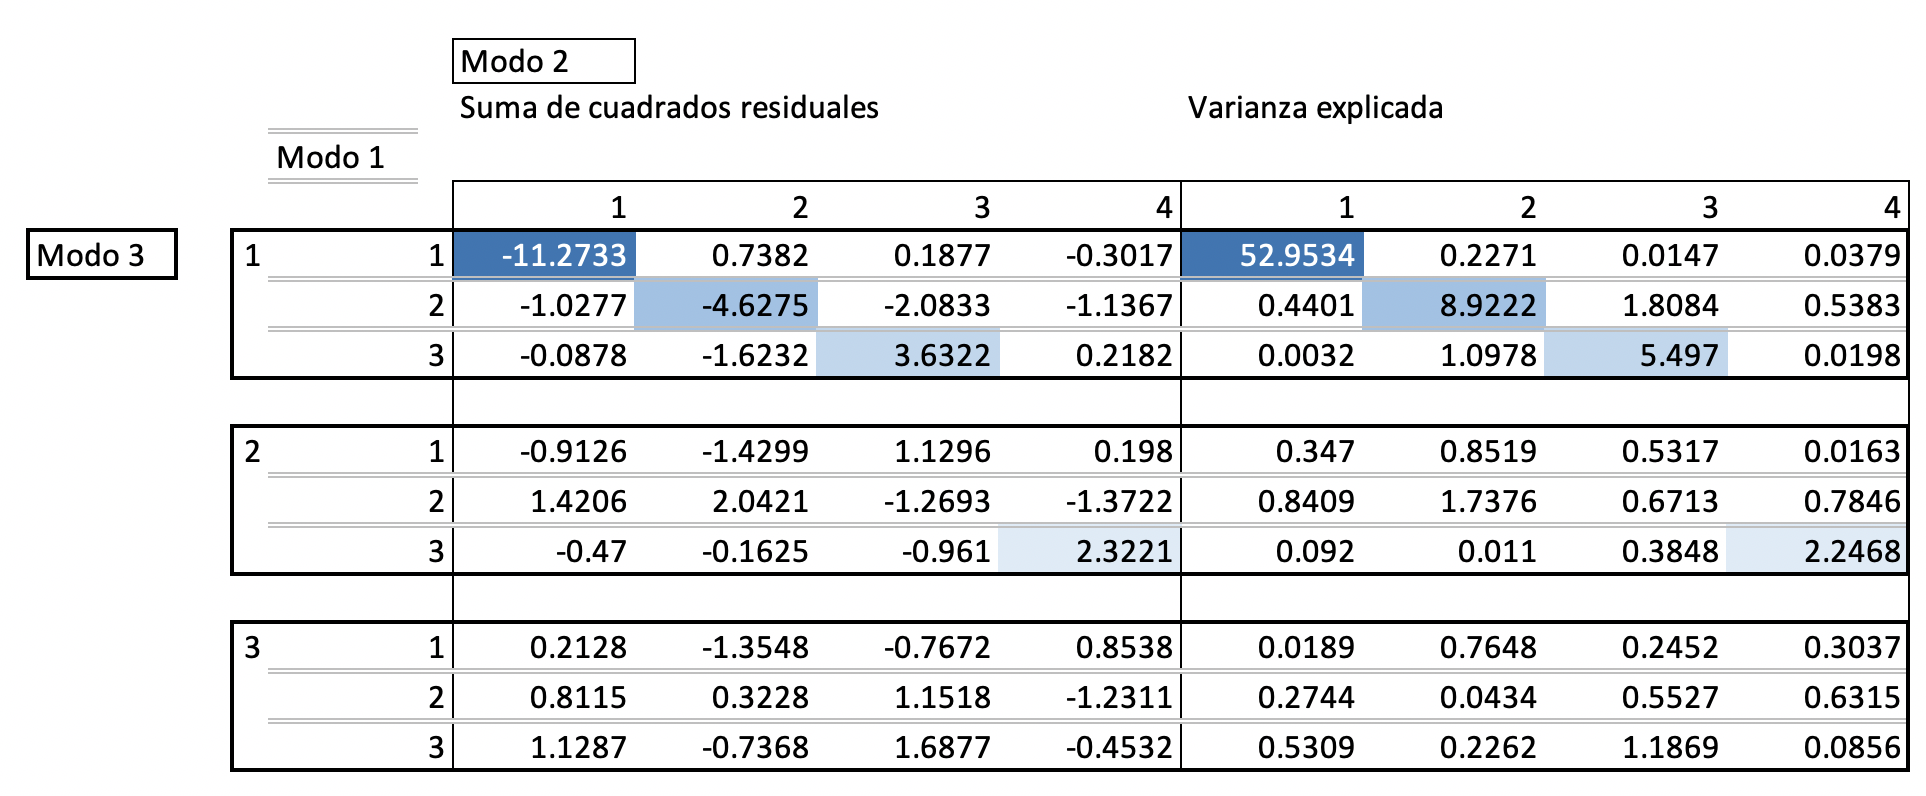
\includegraphics[width=1\linewidth]{core_array}

\caption{Configuración del core array.}

(\#fig:core\_array)
\textbackslash end\{figure\}

\begin{longtable}[]{@{}lrrr@{}}
\caption{Porcentajes de ajuste}\tabularnewline
\toprule
Componentes & Dimensión 1 & Dimensión 2 & Dimensión 3\tabularnewline
\midrule
\endfirsthead
\toprule
Componentes & Dimensión 1 & Dimensión 2 & Dimensión 3\tabularnewline
\midrule
\endhead
1 & 56.313 & 55.5010 & 71.5599\tabularnewline
2 & 17.245 & 13.8817 & 8.5158\tabularnewline
3 & 11.382 & 10.8926 & 4.8642\tabularnewline
4 & 0.000 & 4.6646 & 0.0000\tabularnewline
Total de varianza explicada & 84.940 & 84.9400 & 84.9400\tabularnewline
\bottomrule
\end{longtable}

Adicionalmente, el cuadro muestra el porcentaje del ajuste de varianza total y de cada componente del modelo.

Las coordenadas de las filas, de las columnas y de las repeticiones, así como sus contribuciones correspondientes, se obtienen para biplots posteriores.

\hypertarget{interacciones}{%
\subsubsection{Interacciones}\label{interacciones}}

Finalmente, para poder interpretar las diferentes interacciones más profundas entre lugares, variables medioambientales y estaciones del año, se extraen 4 elementos del \emph{core array}. Se cuenta con la ayuda de gráficos bidimensionales. Esto se logra escribiendo los siguientes argumentos derivados del \emph{core array}:

\begin{longtable}[]{@{}ll@{}}
\caption{Argumentos para interacciones entre variables}\tabularnewline
\toprule
\begin{minipage}[b]{0.16\columnwidth}\raggedright
Argumento\strut
\end{minipage} & \begin{minipage}[b]{0.72\columnwidth}\raggedright
Descripción\strut
\end{minipage}\tabularnewline
\midrule
\endfirsthead
\toprule
\begin{minipage}[b]{0.16\columnwidth}\raggedright
Argumento\strut
\end{minipage} & \begin{minipage}[b]{0.72\columnwidth}\raggedright
Descripción\strut
\end{minipage}\tabularnewline
\midrule
\endhead
\begin{minipage}[t]{0.16\columnwidth}\raggedright
\texttt{P1}, \texttt{P2}\strut
\end{minipage} & \begin{minipage}[t]{0.72\columnwidth}\raggedright
Representaciones de los ejes horizontal (\texttt{*1}) y
vertical (\texttt{*2}) de la primear dimensión. Reciben un
\texttt{integer\ \textgreater{}=\ 1} o \texttt{\textless{}=} el número de elementos que
integran la primera dimensión, además deben cumplir
\texttt{P1\ \textless{}\ P2} (a menos que se retenga un solo componente).\strut
\end{minipage}\tabularnewline
\begin{minipage}[t]{0.16\columnwidth}\raggedright
\texttt{Q1}, \texttt{Q2}
,\texttt{R1},
\texttt{R2}\strut
\end{minipage} & \begin{minipage}[t]{0.72\columnwidth}\raggedright
Aplica de manera análoga a los argumentos \texttt{P*}.\strut
\end{minipage}\tabularnewline
\bottomrule
\end{longtable}

En suma, el criterio para elegir las combinaciones de signos adecuados es considerar los elementos que tengan la varianza explicada más alta, con los elementos de valores residuales con signo positivo.

Luego entonces, conforme a lo señalado en el esquema , el elemento con la varianza explicada más alta es \(52.95\%\) y corresponde a los modos 1, 1, 1 y el signo de la varianza core es negativo (porque la suma de residuos es \(-11.27\)) . El segundo elemento de los modos 2, 2, 1 es \(8.92\%\), también con signo negativo. Le sigue el elemento con modos 3, 3, 1 con \(5.49\%\) de varianza explicada y signo positivo. Finalmente, el cuarto elemento se encuentra en los modos 3,4,2 con \(2.25\%\) de varianza explicada y signo positivo.

Cabe señalar que en los modelos \textbf{Tucker}, los signos del \texttt{core\ array} en conjunto con los de las contribuciones determina la dirección de interacción entre las dimensiones.

Se interpretan las primeras dos configuraciones de los elementos. Notar que en el nuevo código no es necesario pedir las contibuciones:

\begin{Shaded}
\begin{Highlighting}[]
\KeywordTok{TUCKER3}\NormalTok{(}\DataTypeTok{X =}\NormalTok{ var\_cubo,}
        \DataTypeTok{norm =} \OtherTok{TRUE}\NormalTok{,}
        \DataTypeTok{p =} \DecValTok{3}\NormalTok{,}
        \DataTypeTok{q =} \DecValTok{4}\NormalTok{,}
        \DataTypeTok{r =} \DecValTok{3}\NormalTok{,}
        \DataTypeTok{P1 =} \DecValTok{1}\NormalTok{,}
        \DataTypeTok{P2 =} \DecValTok{2}\NormalTok{,}
        \DataTypeTok{Q1 =} \DecValTok{1}\NormalTok{,}
        \DataTypeTok{Q2 =} \DecValTok{2}\NormalTok{,}
        \DataTypeTok{R1 =} \DecValTok{1}\NormalTok{,}
        \DataTypeTok{R2 =} \DecValTok{2}\NormalTok{,}
        \DataTypeTok{coloresf =}\NormalTok{ col\_filas,}
        \DataTypeTok{coloresc =}\NormalTok{ col\_col\_y)}
\end{Highlighting}
\end{Shaded}

\begin{Shaded}
\begin{Highlighting}[]
\NormalTok{knitr}\OperatorTok{::}\KeywordTok{include\_graphics}\NormalTok{(}\StringTok{"interaccion\_var\_1\_2.pdf"}\NormalTok{)}
\end{Highlighting}
\end{Shaded}

\textbackslash begin\{figure\}
\includegraphics[width=1\linewidth]{interaccion_var_1_2}

\caption{Biplots de contribuciones 1 y 2}

(\#fig:elem\_1\_2)
\textbackslash end\{figure\}

\begin{Shaded}
\begin{Highlighting}[]
\NormalTok{knitr}\OperatorTok{::}\KeywordTok{include\_graphics}\NormalTok{(}\StringTok{"interaccion\_var\_1\_2\_mayor.pdf"}\NormalTok{)}
\end{Highlighting}
\end{Shaded}

\textbackslash begin\{figure\}
\includegraphics[width=1\linewidth]{interaccion_var_1_2_mayor}

\caption{Elementos de 1 y 2 con mayor contribución}

(\#fig:elem\_1\_2\_may)
\textbackslash end\{figure\}

Se obtienen los gráficos . El primero muestra la interacción desglosada por dimensiones, mientras que el segundo señala los elementos con mayor contribución.

Continuando con el ejercicio, los siguientes elementos serían:

\begin{Shaded}
\begin{Highlighting}[]
\KeywordTok{TUCKER3}\NormalTok{(}\DataTypeTok{X =}\NormalTok{ var\_cubo,}
        \DataTypeTok{norm =} \OtherTok{TRUE}\NormalTok{,}
        \DataTypeTok{p =} \DecValTok{3}\NormalTok{,}
        \DataTypeTok{q =} \DecValTok{4}\NormalTok{,}
        \DataTypeTok{r =} \DecValTok{3}\NormalTok{,}
        \DataTypeTok{P1 =} \DecValTok{2}\NormalTok{,}
        \DataTypeTok{P2 =} \DecValTok{3}\NormalTok{,}
        \DataTypeTok{Q1 =} \DecValTok{3}\NormalTok{,}
        \DataTypeTok{Q2 =} \DecValTok{4}\NormalTok{,}
        \DataTypeTok{R1 =} \DecValTok{1}\NormalTok{,}
        \DataTypeTok{R2 =} \DecValTok{2}\NormalTok{,}
        \DataTypeTok{coloresf =}\NormalTok{ col\_filas,}
        \DataTypeTok{coloresc =}\NormalTok{ col\_col\_y)}
\end{Highlighting}
\end{Shaded}

\begin{Shaded}
\begin{Highlighting}[]
\NormalTok{knitr}\OperatorTok{::}\KeywordTok{include\_graphics}\NormalTok{(}\StringTok{"interaccion\_var\_3\_4.pdf"}\NormalTok{)}
\end{Highlighting}
\end{Shaded}

\textbackslash begin\{figure\}
\includegraphics[width=1\linewidth]{interaccion_var_3_4}

\caption{Biplots de contribuciones 1 y 2}

(\#fig:elem\_3\_4)
\textbackslash end\{figure\}

\begin{Shaded}
\begin{Highlighting}[]
\NormalTok{knitr}\OperatorTok{::}\KeywordTok{include\_graphics}\NormalTok{(}\StringTok{"interaccion\_var\_3\_4\_mayor.pdf"}\NormalTok{)}
\end{Highlighting}
\end{Shaded}

\textbackslash begin\{figure\}
\includegraphics[width=1\linewidth]{interaccion_var_3_4_mayor}

\caption{Elementos de 1 y 2 con mayor contribución}

(\#fig:elem\_3\_4\_may)
\textbackslash end\{figure\}

\hypertarget{conclusiones}{%
\subsection{Conclusiones}\label{conclusiones}}

Con este manual se intentó mostrar cómo aplicar el modelo Tucker-3 para datos de tres dimensiones. Esta técnica permite fácilmente desglosar las interacciones entre variables que de otra forma solo se podrían obtener agregadamente. Existe mucha investigación por realizar con estas técnicas, con especial atención a datos espaciales.

\hypertarget{bibliografuxeda}{%
\section*{Bibliografía}\label{bibliografuxeda}}
\addcontentsline{toc}{section}{Bibliografía}

\hypertarget{refs}{}
\begin{cslreferences}
\leavevmode\hypertarget{ref-Rodriguez2019}{}%
Rodriguez-Rosa, M. (2019). \emph{KTensorGraphs: Co-Tucker3 Analysis of Two Sequences of Matrices}. \url{https://CRAN.R-project.org/package=KTensorGraphs}

\leavevmode\hypertarget{ref-rodriguez2018}{}%
Rodrı́guez-Rosa, M., Gallego-Álvarez, I., \& Galindo-Villardón, M. P. (2018). Spatio-temporal analysis of economic, social, and environmental issues in the framework of sustainable development in worldwide countries. \emph{Sustainable Development}, \emph{27}(3), 429-447.

\leavevmode\hypertarget{ref-thioulouse2004}{}%
Thioulouse, J., Simier, M., \& Chessel, D. (2004). Simultaneous analysis of a sequence of paired ecological tables. \emph{Ecology}, \emph{85}(1), 272-283.
\end{cslreferences}

\end{document}
